%File: anonymous-submission-latex-2024.tex
\documentclass[letterpaper]{article} % DO NOT CHANGE THIS
\usepackage[submission]{aaai24}  % DO NOT CHANGE THIS
\usepackage{times}  % DO NOT CHANGE THIS
\usepackage{helvet}  % DO NOT CHANGE THIS
\usepackage{courier}  % DO NOT CHANGE THIS
\usepackage[hyphens]{url}  % DO NOT CHANGE THIS
\usepackage{graphicx} % DO NOT CHANGE THIS
\urlstyle{rm} % DO NOT CHANGE THIS
\def\UrlFont{\rm}  % DO NOT CHANGE THIS
\usepackage{natbib}  % DO NOT CHANGE THIS AND DO NOT ADD ANY OPTIONS TO IT
\usepackage{caption} % DO NOT CHANGE THIS AND DO NOT ADD ANY OPTIONS TO IT
\frenchspacing  % DO NOT CHANGE THIS
\setlength{\pdfpagewidth}{8.5in} % DO NOT CHANGE THIS
\setlength{\pdfpageheight}{11in} % DO NOT CHANGE THIS
%
% These are recommended to typeset algorithms but not required. See the subsubsection on algorithms. Remove them if you don't have algorithms in your paper.
\usepackage{algorithm}
\usepackage{algorithmic}

%
% These are are recommended to typeset listings but not required. See the subsubsection on listing. Remove this block if you don't have listings in your paper.
\usepackage{newfloat}
\usepackage{listings}
\DeclareCaptionStyle{ruled}{labelfont=normalfont,labelsep=colon,strut=off} % DO NOT CHANGE THIS
\lstset{%
	basicstyle={\footnotesize\ttfamily},% footnotesize acceptable for monospace
	numbers=left,numberstyle=\footnotesize,xleftmargin=2em,% show line numbers, remove this entire line if you don't want the numbers.
	aboveskip=0pt,belowskip=0pt,%
	showstringspaces=false,tabsize=2,breaklines=true}
\floatstyle{ruled}
\newfloat{listing}{tb}{lst}{}
\floatname{listing}{Listing}
%
% Keep the \pdfinfo as shown here. There's no need
% for you to add the /Title and /Author tags.
\pdfinfo{
/TemplateVersion (2024.1)
}

% DISALLOWED PACKAGES
% \usepackage{authblk} -- This package is specifically forbidden
% \usepackage{balance} -- This package is specifically forbidden
% \usepackage{color (if used in text)
% \usepackage{CJK} -- This package is specifically forbidden
% \usepackage{float} -- This package is specifically forbidden
% \usepackage{flushend} -- This package is specifically forbidden
% \usepackage{fontenc} -- This package is specifically forbidden
% \usepackage{fullpage} -- This package is specifically forbidden
% \usepackage{geometry} -- This package is specifically forbidden
% \usepackage{grffile} -- This package is specifically forbidden
% \usepackage{hyperref} -- This package is specifically forbidden
% \usepackage{navigator} -- This package is specifically forbidden
% (or any other package that embeds links such as navigator or hyperref)
% \indentfirst} -- This package is specifically forbidden
% \layout} -- This package is specifically forbidden
% \multicol} -- This package is specifically forbidden
% \nameref} -- This package is specifically forbidden
% \usepackage{savetrees} -- This package is specifically forbidden
% \usepackage{setspace} -- This package is specifically forbidden
% \usepackage{stfloats} -- This package is specifically forbidden
% \usepackage{tabu} -- This package is specifically forbidden
% \usepackage{titlesec} -- This package is specifically forbidden
% \usepackage{tocbibind} -- This package is specifically forbidden
% \usepackage{ulem} -- This package is specifically forbidden
% \usepackage{wrapfig} -- This package is specifically forbidden
% DISALLOWED COMMANDS
% \nocopyright -- Your paper will not be published if you use this command
% \addtolength -- This command may not be used
% \balance -- This command may not be used
% \baselinestretch -- Your paper will not be published if you use this command
% \clearpage -- No page breaks of any kind may be used for the final version of your paper
% \columnsep -- This command may not be used
% \newpage -- No page breaks of any kind may be used for the final version of your paper
% \pagebreak -- No page breaks of any kind may be used for the final version of your paperr
% \pagestyle -- This command may not be used
% \tiny -- This is not an acceptable font size.
% \vspace{- -- No negative value may be used in proximity of a caption, figure, table, section, subsection, subsubsection, or reference
% \vskip{- -- No negative value may be used to alter spacing above or below a caption, figure, table, section, subsection, subsubsection, or reference

\setcounter{secnumdepth}{0} %May be changed to 1 or 2 if section numbers are desired.

\usepackage{amsmath}
\usepackage{amssymb}
\usepackage{amsthm}
\usepackage{todonotes}
\usepackage{bm}
\usepackage{subcaption}
% \usepackage[ruled]{algorithm2e}

\def\ci{\perp\!\!\!\!\!\perp}

\newtheorem{definition}{Definition}
\newtheorem{proposition}{Proposition}


% The file aaai24.sty is the style file for AAAI Press
% proceedings, working notes, and technical reports.
%

% Title

% Your title must be in mixed case, not sentence case.
% That means all verbs (including short verbs like be, is, using,and go),
% nouns, adverbs, adjectives should be capitalized, including both words in hyphenated terms, while
% articles, conjunctions, and prepositions are lower case unless they
% directly follow a colon or long dash
\title{Title}
\author{
    %Authors
    % All authors must be in the same font size and format.
    Written by AAAI Press Staff\textsuperscript{\rm 1}\thanks{With help from the AAAI Publications Committee.}\\
    AAAI Style Contributions by Pater Patel Schneider,
    Sunil Issar,\\
    J. Scott Penberthy,
    George Ferguson,
    Hans Guesgen,
    Francisco Cruz\equalcontrib,
    Marc Pujol-Gonzalez\equalcontrib
}
\affiliations{
    %Afiliations
    \textsuperscript{\rm 1}Association for the Advancement of Artificial Intelligence\\
    % If you have multiple authors and multiple affiliations
    % use superscripts in text and roman font to identify them.
    % For example,

    % Sunil Issar\textsuperscript{\rm 2},
    % J. Scott Penberthy\textsuperscript{\rm 3},
    % George Ferguson\textsuperscript{\rm 4},
    % Hans Guesgen\textsuperscript{\rm 5}
    % Note that the comma should be placed after the superscript

    1900 Embarcadero Road, Suite 101\\
    Palo Alto, California 94303-3310 USA\\
    % email address must be in roman text type, not monospace or sans serif
    proceedings-questions@aaai.org
%
% See more examples next
}

%Example, Single Author, ->> remove \iffalse,\fi and place them surrounding AAAI title to use it
\iffalse
\title{My Publication Title --- Single Author}
\author {
    Author Name
}
\affiliations{
    Affiliation\\
    Affiliation Line 2\\
    name@example.com
}
\fi

\iffalse
%Example, Multiple Authors, ->> remove \iffalse,\fi and place them surrounding AAAI title to use it
\title{My Publication Title --- Multiple Authors}
\author {
    % Authors
    First Author Name\textsuperscript{\rm 1},
    Second Author Name\textsuperscript{\rm 2},
    Third Author Name\textsuperscript{\rm 1}
}
\affiliations {
    % Affiliations
    \textsuperscript{\rm 1}Affiliation 1\\
    \textsuperscript{\rm 2}Affiliation 2\\
    firstAuthor@affiliation1.com, secondAuthor@affilation2.com, thirdAuthor@affiliation1.com
}
\fi


\begin{document}

\maketitle

\begin{abstract}
	% TODO: Needs to be shortened.
	% In Pearl's framework, the initial step for performing a causal analysis
	% involves determining the causal structure between the variables from
	% data typically in the form of a Directed Acyclic Graph (DAG) or an
	% Structural Equation Model (SEM). This procedure, known as \emph{causal
	% discovery}, has been extensively studied for both DAGs and SEMs. While
	% numerous automated algorithms exist for estimating DAGs from datasets,
	% their application in applied fields remain limited, possibly due to a
	% lack of confidence in these algorithms stemming from them making
	% obvious mistakes, and the difficulties in choosing the right algorithm
	% for a given dataset. Consequently, in applied disciplines, these DAGs
	% are predominantly constructed manually based on domain expertise. Due
	% to being constructed by hand, it is vital that the fit of these models
	% are tested against data and the models are potentially modified to
	% acheive a better fit. On the other hand, in the field of SEMs models
	% are typically constructed manually through an iterative process of
	% assessing fit and modifying the model according to that. This process
	% is commonly known as \emph{Specification Search} where methods like
	% \emph{modification indices} combined with expert knowledge can be used
	% to guide this modification process. In the case of DAGs, although there
	% are tests to assess the global fit of a model by combining the tests
	% using implied conditional independencies of the model, but there are no
	% methods that can guide our modification process. In this paper, we
	% present a simple modification process aimed at helping researchers in
	% manually constructing or modifying DAGs outputted by an algorithm. This
	% modification process is based on using a (conditional) measure of
	% association between variables in the model to assess potential edges
	% that best explains unexplained correlation between variables which the
	% researcher specifies the direction of this edge. In the case of
	% continuous or discrete variables, the effect size measures of local
	% tests can be used as this measure of association, however for mixed
	% data there is no such measure. We present a measure of association
	% based on canonical correlations for mixed data. We also present a
	% graphical web-tool that can assist researchers in iteratively modifying
	% and constructing their DAGs. We theoretically show that in the presence
	% of an oracle, this iterative modification process is consistent in
	% recovering the true DAG. Emprically, we show that using the mixed data
	% measure of association, the modification process performs comparably to
	% PC and Hill-Climb Search algorithms if the user is able to correctly
	% identify the direction of the edge in one out of three cases.
\end{abstract}

\section{Introduction}

Many questions in science center around understanding the cause and effect
relationships between variables, as it can reveal the underlying mechanisms for
the observed phenomena and inform effective interventions or policy decisions.
\emph{Causal Discovery} methods aim to find the underlying causal structure
among random variables from a given dataset. The problem of causal discovery
has been studied in both Directed Acyclic Graphs (DAGs) and Structural Equation
Models (SEM) literatures with different approaches. In the DAG literature, the
focus has been on developing automated algorithms that can learn the causal
structure from a given observational or interventional dataset, whereas in the
SEM literature the focus has on developing tools to help researchers construct 
models manually or modify manually constructed models.

% To perform any causal effect identification or estimation using Directed
% Acyclic Graphs (DAGs) or Structural Equation Models (SEMs), researchers need to
% first construct a causal structure commonly known as DAG or path diagram. This
% process of constructing the casual structure from data is known as \emph{Causal
% Discovery}. In the field of DAGs, plenty of algorithms have been developed to
% automatically construct DAGs from data. These algorithm takes different
% approaches to causal discovery such as Constraint-based algorithms such as PC
% and Fast Causal Infenrece (FCI) where the algorithm tries to match the
% conditional independences in the data to the ones impled by the model,
% score-based methods such as Hill-Climb Search, Greedy Equivalence Search (GES)
% where the algorithm tries to find a model that has the best score given some
% scoring metric, and continuous optimization where the problem is formulated as
% a constrained optimization problem such as No Tears.

In the DAG literature, many automated algorithms have been developed for causal
discovery such as constraint based methods like PC \citep{Spirtes2001} and FCI
\citep{Spirtes2000}, score-based methods like Hill-Climb Search, Greedy
Equivalence Search \citep{Chickering2002}, and optimization based methods.
However, the adaption of these algorithms in applied fields remain limited
\citep{Tennant2020}. In applied fields, researchers typically prefer to
construct these DAGs manually based on their domain knowledge. We hypothesize
that this preference towards manual DAG construction stems from the following
difficulties in applying causal discovery methods:

\begin{enumerate}
	\item \textbf{Difficult to trust: } Even though most of these algorithms
		have asymptotic theory proving them to be consistent, their
		finite sample properties is not well understood. In real
		setting with finite samples, these algorithms can make obvious
		mistakes. As a result of this, researchers have to rely on
		post-hoc modification of the output of these algorithms
		using either their domain knowledge or assisted by model testing
		methods.
	\item \textbf{Algorithms output Markov Equivalence Class (MEC):} Given an 
		observational dataset, multiple causal structures can be
		faithful to it. As a result, using only observational datasets,
		these algorithms can only get to the MEC such as Completed
		Partially Directed Acyclic Graph (CPDAG) or a Partial Ancestral
		Graph (PAG) where not all the edges are directed. However, as
		most of the methods developed for downstream tasks such as
		identification or casual effect estimation assume the knowledge
		of a DAG. To orient these MECs to a DAG, researchers have to
		either rely on their domain expertise, or make further
		assumption to utilize a pairwise orientation method.
	\item \textbf{Difficult to choose appropriate algorithm and
		hyperparameters:} All the algorithms have the same goal with
		all of them having similar asymptotic properties. However, the
		finite sample properties of these methods vary depending on the
		choices that we make. For example, the choice of the
		conditional independence (CI) test being used for
		constraint-based method depends on the dataset, similarly for
		the scoring method for score-based methods. With no obvious way
		to test the impact/performance of these choices on a given
		dataset, it becomes quite hard to chose the optimal algorithm
		for a given dataset.
\end{enumerate}

On the other hand, in the field of Structural Equation Models (SEMs), a lot
more focus has been put on methods to help researchers draw models manually
along with integrating their expertise. Researchers typically come up with an
initial model based on their domain knowledge, and then use various tools to
guide them in making modifications to this initial model. This process of
constructing models is commonly known as \emph{Specification Search}. A
commonly used method for suggesting potential modifications to the SEM is
\emph{modification indices}. Given a specified model, modification indices
tries to find potential modifications to the model that improve the model's fit
to the data best. Based on the suggestions from this method along with their
domain expertise, the researcher can then choose the most optimal modification
for their model.

\todo[inline]{Other methods: Modification indices and Lagrange Multiplier tests to
selectively add edges And using Wald test or z statistics (also known as
critical ratios) for removing edges.}

As it is evident that researchers also draw DAGs by hand and even if they use
an algorithm, the need to make some post-hoc adjustments to the model, in this
paper we present a tool to assist researchers in making these adjustments
somewhat inspired by modification indices. In the case of DAGs, global testing
methodology does exist such as Shipley test, that can combine local structure
tests into a single p-value test. However, this does not give us a way to make
modifications to our model. A possible way to do this by checking which of
these local tests are violated. However, this approach can quickly become
diffult as the size of the network increases. For example, the popular alarm
network implies $x$ condition independence statements.

% One of the drawbacks of these global fit metrics is that they do not only test
% for the structure but also the fitted parameterization.

Our proposed approach uses a measure of association to find correlated variables
in the data that are not explained by the current model. Using the measure, we 
can rank the edge that can lead to the highest explanation of the observed 
correlation. Based on this information, the user can select a potential edge
and based on their expert knowledge decide the direction of the edge.

% We present a similar procedure for modifying DAGs based on expert knowledge and
% measure of association. We first use the measure of association to test whether
% the association observed in the data is explained by the model structure. We
% can not directly use the local CI tests to make modifications because that
% would give way too many independencies and we have no way to rank them. Based
% on this testing, we suggest adding edges by ranking them by the most
% unexplained association between variables. The researcher can then use expert
% knowledge to decide the direction of the edge between the variables.

Our main contributions in this papers are as follows:
\begin{enumerate}
	\item We present a measure of (conditional) association for mixed data
		based on canonical correlations. This measure of association
		generalizes the widely used partial correlation to mixed data
		setting.
	\item Using this association measure, we present a procedure to suggest
		potential new edges, or edge removals in the model. The user
		gets to decide the direction of the new edge based on their
		expertise.
	\item Lastly, we present a web-browser based tool to allow researchers
		to apply this method to their own datasets.
\end{enumerate}

\begin{figure}
		\centering
		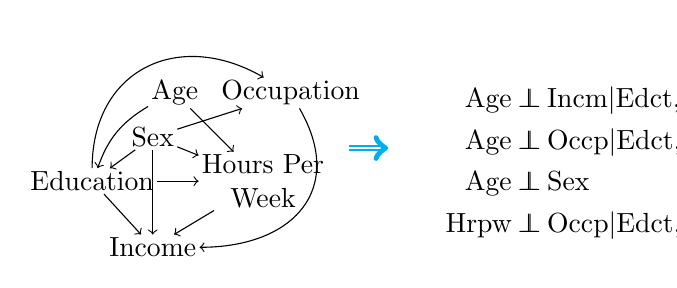
\begin{tikzpicture}
			\begin{scope}[xshift=-2.5cm, yshift=0.7cm, scale=0.7]
			\tikzstyle{every node}=[align=center, inner sep=1pt]
				\node (sex) at (-0.7, -0.8) {Sex};
				\node (age) at (-0.3, 0) {Age};
				\node (ed) at (-1.8, -1.6) {Education};
				\node (occ) at (1.8, 0) {Occupation};
				\node (hrpw) at (1.3, -1.6) {Hours Per \\ Week};
				\node (income) at (-0.7, -2.8) {Income};
			
				\draw[->]  (age) to[bend right=20] (ed);
				\draw[->]  (sex) to (ed);
				\draw[->]  (age) to (hrpw);
				\draw[->]  (ed) to (hrpw);
				\draw[->]  (sex) to (hrpw);
				\draw[->]  (ed) to (income);
				\draw[->]  (hrpw) to (income);
				\draw[->]  (occ) to[out=300, in=0, looseness=1.4] (income.east);
				\draw[->]  (sex) to (income);
				\draw[->]  (ed) to[out=90, in=150, looseness=1.3] (occ);
				\draw[->]  (sex) to (occ);	
			\end{scope}
			\begin{scope}[xshift=-3cm]
				\draw[thick, ->, double, cyan] (2.5,0) -- (3,0);
				\node[rectangle, align=center, inner sep=1pt] at (5, 0) {
					\begin{minipage}{.2\textwidth}
						\begin{equation*}
							\begin{split}
								\textnormal{Age} &\ci \textnormal{Incm} \rvert \textnormal{Edct, Hrpw, Sex} \\
								\textnormal{Age} &\ci \textnormal{Occp} \rvert \textnormal{Edct, Sex} \\
								\textnormal{Age} &\ci \textnormal{Sex} \\
								\textnormal{Hrpw} &\ci \textnormal{Occp} \rvert \textnormal{Edct, Sex} \\
							\end{split}
						\end{equation*}
					\end{minipage}
					};
			\end{scope}
		\end{tikzpicture}
		\caption{\todo[inline]{Show a full example of testing using this model}}
\end{figure}

The rest of the paper is structured as follows. In
Section~\ref{sec:background}, we give a background on the measures of
association for various data types. In Section~\ref{sec:mixed_association}, we
present our method for computing mixed data association. In
Section~\ref{sec:modification}, we present how to use this method to rank the
modifications, and lastly in Section~\ref{sec:empirical}, we show some
empirical analysis on how well this modification process works.

\section{Background}
\label{sec:background}
We represent uni-dimensional variables as $ X $ and multi-dimensional variables
as $ \bm{Z} $. All the variables are considered to be any mix of continuous,
ordinal, or categorical unless specified explicitly.

We consider the case of estimating association between $ X $ and $ Y $ is the
presence of a set of conditioning variables $ \bm{Z} = Z_1, \cdots, Z_k $,
potentially being an empty set $ \bm{Z} = \emptyset $. We use $ \rvert \bm{Z}
\rvert $ to denote the cardinality of the set of variables $ \bm{Z} $. We
consider various scenarios where the variables $ X $, $ Y $ and $ \bm{Z} $
could be either discrete, ordinal, or continuous. With mixed data, we mean an
arbitrary mix of variable types among $ X $, $ Y $, and $ \bm{Z} $.

We consider the problem of estimating the partial (or conditional) association
between $ X $ and $ Y $ in the presence of the conditioning set $ Z $. When $ Z
= \emptyset $, this is equivalent to the marginal association between $ X $ and
$ Y $.

\todo[inline]{Add more notation as they come}

\subsection{Measures of (Conditional) Association}
As our DAG construction procedure relies on a measure of conditional
association between variables, in this section we list out some of the already
known measures for specific data types. These measure of associations are
typically the effect size of various conditional indepdnence tests but they
don't need to be. However, there are no generalized measure of association for
mixed data, that we propose in the next section. This is by no means an
exhaustive list, rather just to give an idea of what can be done.

\paragraph{Both $ X $ and $ Y $ are continuous}
Where there are no conditional variables, $ \bm{Z} = \emptyset $, Pearson's
correlation coefficient can be used as a measure of association between the
variables. This does make various assumptions such as linearity between the
variables, normal distribution for $ X $ and $ Y $, and homoscedasticity.

In the case when $ \bm{Z} \neq \emptyset $, then partial correlations can be
used. This requires using two linear regression models: $ E_X: X \sim \bm{Z} $
and $ E_Y: Y \sim \bm{Z} $. Then computing the residuals using these two
regressions as: $ R_X = X - E_X(\bm{Z}) $ and $ R_Y = Y - E_Y(\bm{Y}) $. After
this a simple correlation coefficient can be computed between $ R_X $ and $ R_Y $.

\paragraph{All $ X $, $ Y $, and $ \bm{Z} $ are discrete}

In the case of discrete variables, Cramer\'s V has been typically used as a
measure of association. When there are no conditional variables, $ \bm{Z} = \emptyset $,
Cramer\'s V can be computed directly from the contingency table.

However, when conditional variables are present, we can iterate over all
possible combinations of the conditional variables, compute the Cramer\'s V and
then lastly combine them together. 

\todo[inline]{Is it even possible}

\paragraph{$ X $ is ordinal and $ Y $ is continuous}
Polyserial Correlation

When $ \bm{Z} = \emptyset $, ordinal variable can be assumed to be coming from
a thresholded normal distribution, estimate the thresholds and latent variable
to compute the correlation coefficient.

\paragraph{$ X $ and $ Y $ are ordinal}
Polychoric Correlation

\section{Measure of Association for Mixed Data}
\label{sec:mixed_association}

In this section, we develop a novel (conditional) measure of association for
mixed data. The presented measure extends partial correlation to mixed data by
combining a mixed-data residualization method with a multivariate measure of
association.

Given two variables $ X $ and $ Y $, and a set of conditional variables $
\bm{Z} $, we are interested in computing the conditional association, $ \rho(X,
Y; Z) $. As our measure is based on residulaization, we start by computing the
residuals for $ X $ and $ Y $ using the $ \bm{Z} $ as the predictor variables.
We use the mixed data residualization approach from \citet{Ankan2023}. We
consider each variable type separately and repeat the following steps for both
$ X $ and $ Y $:

\begin{enumerate}
	\item $ X $ is continuous: We start by training a regression model, $
		E_X: X \sim \bm{Z} $. Next we take the predictions from this
		model $ \hat{x} = E_X(\bm{Z}) $ and lastly the residuals are
		computed as the difference between the true and the predicted
		values.
		$$ R_X = X - \hat{x} $$
	\item $ X $ is ordinal: We start by training a probability estimator, $
		p_X: X \sim \bm{Z} $, and take probability predictions from it
		$ \hat{p}_X: p_X(\bm{Z}) $. Then we compute the residuals as follows:
		$$ R_X = $$
	\item $ X $ is categorical: We again start by training a probability estimator
		$ p_X: X \sim \bm{Z} $, and take the probability estimates from it $ \hat{p}_X: p_Z(\bm{Z}) $.
		Next, we one-hot encode the categorical variable and then compute the residuals
		as follows:
		$$ R_X $$
\end{enumerate}

Here, users can choose the type of estimator that they want to use. There are
single estimators such as Random Forest or XGBoost that can work for both the
probability estimates and regression estimates. Or users can also choose
different estimators such as variants of linear regression for computing the
residuals. After the above steps are repeated for both $ X $ and $ Y $, we end
up with two residual matrices: $ R_X $ and $ R_Y $. The type of the variable
determines the shape for these matrices, i.e., if the variable is continuous we
get a residual matrix of shape $ ( n \times 1 ) $ and if the variable is
categorical we have a residual matrix of shape $ ( n \times (k-1)) $ (where one
of the dummy encoded variables is dropped to avoid multicollinearity)

Now, we have the two residuals and we need a measure to quantify the
association between these residuals. As the residuals are matrices, we can
treat them as sets of random variables, and in multivariate analysis canonical
correlations have been used to quantify association between two sets of
variables. Canonical correlations are generalization of correlations to
multi-dimensional variables where they try to find linear combinations of the
given sets of variables that maximize the correlation between them.

\begin{definition}
	Given two sets of random variables $ \bm{U} = (U_1, U_2, \cdots, U_p) $
	and $ \bm{V} = (V_1, V_2, \cdots, V_q) $, canonical correlation between
	them, $\rho(\bm{U}, \bm{V}) $ is defined as:
		
	\begin{equation}
		\rho(\bm{U}, \bm{V}) = \sup_{a, b} \frac{a^T \Sigma_{\bm{U}\bm{V}} b}{\sqrt{a^T \Sigma_{\bm{U}\bm{U}} a} \sqrt{b^T \Sigma_{\bm{V}\bm{V}} b}}
	\end{equation}

\end{definition}
	
	Canonical correlations try to find linear transformations $ a $ and $ b
	$ of $ \bm{U} $ and $ \bm{V} $ such that the correlations between the
	columns of $ a^T \bm{U} $ and $ b^T \bm{V} $ is maximized. The
	individual columns of $ a^T \bm{U} $ and $ b^T \bm{V} $ are
	independent. In the case when $ \rvert U \rvert = \rvert V \rvert = 1$,
	canonical correlations are equivalent to Pearson's correlation
	coefficient.

Many measures of association based on canonical correlation are also available such as:
\begin{itemize}
	\item Wilks' Lambda: $ \Lambda = \prod (1 - \phi_i^2) $
	\item Roy's Largest Root: $ \theta = \phi_{\max}^2 $
	\item Pillai's Trace: $ \tau = \sum \phi_i^2 $
\end{itemize}

We use Pillai's Trace in this paper. \todo[inline]{Why?}.

This measure of association has many of the desired properties:

\begin{enumerate}
	\item Is bounded between $ 0 $ and $ 1 $, with $ 0 $ representing no association and $ 1 $ representing a perfect linear relationship.
	\item Is independent of the sample size.
	\item As canonical correlation finds linear transformations, the measure is independent of the one-hot encoding scheme used for categorical variables.
	\item In the case of both continuous variables, it is equivalent to partial correlations.
	\item For both discrete variables, the measure is connected to Cramers\' V, a well know effect size measure for discrete variables.
\end{enumerate}

\section{Using measure of association for modifying DAGs}
\label{sec:modification}

Any two variables in a DAG that do not have an edge between them imply a
conditional independence test that is they are independent given the parents of
both the variables, $ X \ci Y | pa(X) \cup pa(Y) $. In the case of model
testing, a CI statement like this can be used to check whether the assumption
of the model holds in the data or is violated. For mixed data, a few different
CI tests have been proposed such as likelihood-ratio based, and residualization
based. However, if we just use the CI test to check the p-value we cannot use
it to find the modification that is able to improve the score the most. We can
however use the measure of association to check which assocation between the
variables in the data is not explained by the model. Using this the expert can
decide to add an edge between the variables but will need to choose the
direction of the edge.

The idea behind using the measure of association for modifying DAGs is inspired
by modification indices in SEM. 

Theorem - If we have access to an oracle that can give all correct results, 
the algorithm above is consistent.

\section{Web Tool}
\label{sec:web}
Based on the approach outlined in the previous section, we built a web-based
tool that researchers can upload their dataset to and apply this method to
interactively draw models. Users can start by uploading their datasets. The web
interface should then automatically show them all the correlated variables in a
graphical representation. The red colored edges represent potential new edge
between the variables.

\todo[inline]{List some of the features of the online platform}

% \begin{figure}
% 	\centering
% 	\begin{subfigure}{0.5\textwidth}
% 		\includegraphics[scale=0.25]{../../presentations/2024_05_das/2.png}
% 	\end{subfigure}%
% 	\begin{subfigure}{0.5\textwidth}
% 		\includegraphics[scale=0.25]{../../presentations/2024_05_das/5.png}
% 	\end{subfigure}
% 	\caption{Screenshots of the web-tool. \todo[inline]{Insert screenshots of the web-tool}}
% \end{figure}

\section{Empirical Analysis}
\label{sec:empirical}

We analyzed the performance of this manual approach by comparing it with two
automated algorithms: PC and Hill-Climb Search. For the comparison we use
simulated data from a known DAG and compare how well the algorithm is able to
recover the original model using two metrics: Structural Hamming Distance (SHD)
and Structural Intervention Distance (SID). To simulate the data, we start with
a randomly generated DAG and use linear models with random effects to generate
the data. We repeat the data generation $ 30 $ times for each density value for
the DAG. As both PC and Hill-Climb Search can only give us a CPDAG, we compare
the orientation of these CPDAG which result in the best and worst case scores
on SHD and SID. This procedure is outlined in Algorithm 1.

\todo[inline]{Add the algorithm}

To simulate an expert using this assisted model construction approach, we start
with an empty model and take a greedy approach to add edges to this model. At
any point, we select the pair of variables that has significant correlation and
the highest unexplained correlation, i.e., highest conditional association. We
then use an oracle to decide the direction of the edge between the variables.
Given an accuracy of the oracle, $ \alpha $, the oracle either gives the
correct direction, incorrect direction, or returns None representing that it
does not know the direction.

\begin{equation}
	\begin{split}
		x &= \textnormal{rand}([0, 1]) \\
		O(\alpha) &= \begin{cases} 
			M \rightarrow Y, & \textnormal{if  } x <= \alpha \\
			\textnormal{rand}(M \rightarrow Y, M \leftarrow Y, None) & \textnormal{otherwise} \\
				\end{cases} \\
	\end{split}
\end{equation}

If the oracle returns None for any pair of variables, an edge between this pair
is not suggested to the oracle in future iterations. We also make sure that
only edges which do not form a cyclic in the graph are used to select the next
potential edge. After adding each edge, we also check if the p-value of any
existing edge shows independence. If that happens we remove that edge and
blacklist that edge, i.e., that edge is not prompted again during the run of
the algorithm. We repeat this procedure till the model explains all
correlations between the variables. There is a possibility that this greedy
expert gets stuck at incorrect graph structures as it does not do any
backtracking to fix its earlier mistakes. This procedure is outlined in the
Algorithm.
\todo[inline]{Add the algorithm}

\subsection{Results}
\begin{figure}
	\begin{subfigure}{0.5\textwidth}
		\centering
		\includegraphics{../code/plots/shd_ribbon.pdf}
		\caption{}
	\end{subfigure}
	\begin{subfigure}{0.5\textwidth}
		\centering
		\includegraphics{../code/plots/sid_ribbon.pdf}
		\caption{}
	\end{subfigure}
	\caption{Comparison of PC and Hill-Climb Search algorithms against
		manually drawn DAGs using the assistance method. As PC and
		Hill-Climb Search return the Markov Equivalence Class (MEC), we
		use the best and worst scoring orientation of the MEC to get
		the range of values. The human drawn values are done for
		multiple accuracy values of the oracle.}
\end{figure}

\subsection{Using Large Language Models as Experts}
A lot of recent work has focused on finding pairwise causal direction among
variables using Large Language Models. In this analysis, instead of using the
oracle to decide the direction of edges, we used GPT4 to give us the direction
of the edges based on description of the variables. As GPT4 has already
memorized many of these models, we encoded the variable names using a random
string and provided the description of the variable to let it decide the
direction of the edge.

\section{Conclusions}

\bibliography{references}
\end{document}
